\begin{frame}[parent={ie:agenda}, hasnext=true, hasprev=false]
	\frametitle{Simulação de processos}

	\begin{block:concept}{Modelos de simulação}
		Abordagem para realizar a execução do modelo de processo sem utilizar 
		recursos, pessoas e ferramentas reais.
	\end{block:concept}

	
	\begin{block:fact}{Motivação}
		\begin{itemize}
			\item Analisar o comportamento de processos complexos.
			\note{
				\textbf{Sistemas dinâmicos complexos:}
				\begin{itemize}
					\item Entender a complexidade estática não é o mesmo que entender a complexidade
					dinâmica dos processos.
				
					\item Processos não são determinísticos (possuem várias opções) e muitas vezes
					são probabilísticos.
				\end{itemize}
			}
				
			\item Custo mais baixo que abordagens usuais para análise da dinâmica de processos.
			\note{
				
				\textbf{Avaliação:}
				Método usual envolve a condução de estudos experimentais (estudos de casos,
				experimentos controlados) e analisar os resultados desses estudos, o que demanda
				tempo e recursos (financeiros e humanos) consideráveis.
			}
		\end{itemize}
	\end{block:fact}
	
	\note{ 
		
		\textbf{Moral da história:}
		Desta forma, simulação de processos de software apresenta-se como um instrumento
		importante para auxiliar a tomada de decisões durante o gerenciamento de projetos de
		software.
	}
\end{frame}


\begin{frame}[hasnext=true, hasprev=true]
	\frametitle{Simulação de processos}

	\begin{block:fact}{}
		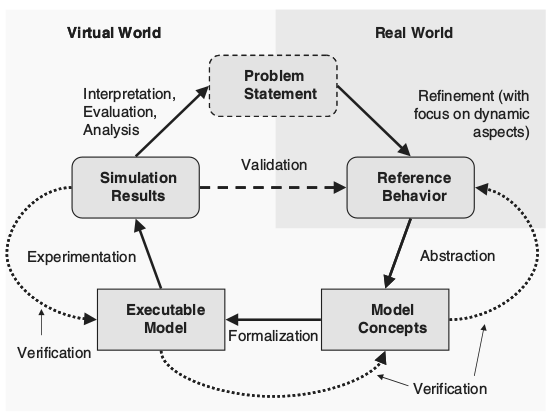
\includegraphics[width=\textwidth]{simulation-modeling-aspects}
		\cite{Muller-Pfahl:2008}
	\end{block:fact}
\end{frame}


\begin{frame}
	\frametitle{Simulação de processos}
	\framesubtitle{Formulação do problema}
	
	\begin{block:concept}{Definição}
		Estabelece o objetivo do modelo de simulação (propósito) e define o escopo
		das atividades de modelagem.
	\end{block:concept}
	
	\begin{block:concept}{Características~\cite{Kelner-etal:1999}}
		\textbf{Propósito}
		\begin{itemize}
			\item Gestão estratégica, operacional, planejamento e controle
			\item Melhoria de processo, adoção de tecnologia
			\item Compreensão do processo, treinamento
		\end{itemize}
		
		\textbf{Escopo}
		\begin{itemize}
			\item Fase do ciclo de vida em que é aplicável
			\item Projeto
			\item Diversos projetos em paralelo
			\item Linha de produto
		\end{itemize}
	\end{block:concept}
\end{frame}


\begin{frame}
	\frametitle{Simulação de processos}
	\framesubtitle{Comportamento de referência}
	
	\begin{block:concept}{Definição}
		Comportamento de referencia captura a variação (dinâmica, dependente de
		tempo) de atributos	importantes de entidades do elemento tratado pela simulação.
		\note{
			Identifica elementos de saída do modelo, permitindo a comparação com
			comportamento observável no mundo real.
		}
	\end{block:concept}
	
	\begin{block:fact}{Exemplos}
		\begin{itemize}
			\item Qualidade
			\item Esforço
			\item Custo
			
			\item Gestão operacional, planejamento e controle
			\item Melhoria de processo
			\item Adoção de tecnologia
			\item Compreensão do processo
			\item Treinamento
		\end{itemize}
	\end{block:fact}
\end{frame}


\begin{frame}
	\frametitle{Simulação de processos}
	\framesubtitle{Conceitos do modelo / Modelagem}
	
	\begin{block:concept}{Definição}
		Abstração de comportamentos observados na realidade, capturando conhecimento
		implícito ou tácito.
	\end{block:concept}
	
	\begin{block:fact}{}
		\begin{itemize}
			\item Modelos existentes de processo, qualidade e recursos.
			\item Regras de decisão (implícitas ou explícitas).
			\item Padrões de comportamento observáveis.
			\item Fluxos de informações organizacionais.
			\item Políticas
		\end{itemize}
	\end{block:fact}
\end{frame}



\begin{frame}
	\frametitle{Simulação de processos}
	\framesubtitle{Modelo de simulação}
	
	\begin{block:concept}{Definição}
		Transformação do modelo de processo em um modelo executável.
		\note{
			Deve-se buscar alinhamento entre a linguagem utilizada para definir o
			modelo de processo e a linhagem do modelo executável. Por exemplo, BPMN.
		}
	\end{block:concept}
\end{frame}


\begin{frame}
	\frametitle{Simulação de processos}
	\framesubtitle{Execução e calibração do modelo}
	
	\begin{block:concept}{Definição}
		Execução do modelo, obtendo-se resultados úteis para tratar o objetivo. Todavia,
		antes deve ocorrer a calibração dos parâmetros do modelo de simulação com
		dados reais.
	\end{block:concept}
\end{frame}


\begin{frame}
	\frametitle{Simulação de processos}
	\framesubtitle{Técnicas para simulação}
	
	\begin{block:concept}{Técnicas}
		\begin{itemize}
			\item Sistema de eventos discretos
			\note{
				Modelo baseado em evento atualiza os valores das variáveis do modelo
				conforme ocorrem eventos.
			}
			\item Sistema dinâmico
			\note{
				Modelo contínuo atualiza o valor das variáveis do modelo de acordo
				com um conjunto bem definido de equações, considerando passos precisos
				e equidistantes de tempo.
				
				Representado por equações diferenciais que, durante a simulação, são
				integradas numericamente.
			}
			\item Híbridos
		\end{itemize}
	\end{block:concept}
\end{frame}


\begin{frame}
	\frametitle{Simulação de processos}
	\framesubtitle{Exemplo:ISDMeLO}
	
	\begin{block:fact}{Simulação do ISDMeLO}
			Processo para desenvolvimento de objetos de aprendizagem segundo ADDIE, ciclo de
			vida em batelada (``cascata'').
	\end{block:fact}
	
	\begin{block:fact}{Características da simulação}
		\begin{itemize}
			\item Sistema de eventos discretos
			\item Ferramenta utilizada: Arena
		\end{itemize}
	\end{block:fact}
\end{frame}


\begin{frame}
	\frametitle{Simulação de processos}
	\framesubtitle{Limitações}
	
	\begin{block:fact}{Limitações}
		\begin{itemize}
			\item Qualidade dos resultados da simulação depende da qualidade do modelo
			e dos valores atribuídos às variáveis.
			\begin{itemize}
				\item Valores devem ser precisos e refletir o cenário real.
			\end{itemize}
			
			\item Dificuldade em definir bons modelos.
		\end{itemize}
	\end{block:fact}
\end{frame}
